\documentclass[11pt]{article}
\usepackage[margin=1in]{geometry}
\usepackage{amsmath}
\usepackage[version=4]{mhchem}
\usepackage[T1]{fontenc}
\usepackage{lmodern}
\usepackage[authoryear,round]{natbib}
\usepackage{graphicx}
\usepackage{float}
\usepackage{url}

\title{Precession Phase Organises the Timing and Direction of DO-Like Asian Monsoon Transitions}
\author{}
\date{}

\begin{document}
\maketitle

\section*{Abstract}

Millennial-scale climate variability (MCV) is a prominent feature of glacial climates, but whether orbital forcing organizes the timing of individual abrupt transitions---beyond modulating overall variance amplitude---remains unclear. Here we test this question using 196 objectively identified weak- and strong-monsoon starts from the Chinese speleothem composite over the past 640\,kyr. Rayleigh tests reveal significant and opposite precession-phase clustering: strong monsoon starts peak near precession-index minima (21.9$^\circ$), while weak starts cluster in the opposite half-cycle (225.3$^\circ$). A history-conditioned binned Poisson model shows that precession-phase information persists after controlling for same-type event history, composite sampling resolution, LR04 benthic $\delta^{18}$O, and atmospheric CO$_2$ (strong starts: LR = 19.74, $p=5.2\times10^{-5}$, 0.150 bits/event; weak starts: LR = 14.52, $p=7.0\times10^{-4}$). The result is stable across bin widths, detection windows, and age-uncertainty perturbations. We interpret this as precession-phase organization of abrupt monsoon-transition probability, superimposed on slower glacial background modulation.

\section*{Introduction}

Millennial-scale climate variability (MCV) is a major expression of abrupt climate change in glacial climate systems. Its canonical manifestation is the Dansgaard--Oeschger (DO) sequence in Greenland ice cores, where rapid stadial--interstadial transitions record major reorganizations of the North Atlantic climate system \citep{rasmussen2014stratigraphic}. Yet MCV was not confined to Greenland. Marine, ice-core, and speleothem archives show that abrupt millennial variability occurred across multiple Pleistocene glacial cycles and was expressed in both high-latitude and low-latitude monsoon systems \citep{barker2011800, sun2021persistent, hodell20231}. Speleothem records provide a particularly powerful archive because their U--Th chronologies allow abrupt hydroclimate changes to be compared directly with ice-core event sequences. During the last glacial period, independently dated speleothem records indicate that abrupt Greenland warmings were accompanied by near-synchronous hydroclimate shifts in monsoon and mid-latitude regions \citep{corrick2020synchronous}. Such speleothem transitions can therefore be treated as precisely dated DO-like Asian monsoon expressions of MCV.


The intensity and occurrence of MCV were strongly conditioned by the slowly evolving background climate state. Proxy syntheses and model experiments indicate that abrupt millennial-scale variability was favoured under intermediate glacial conditions, whereas interglacial and fully glacial end-member states were comparatively unfavourable for the MCV \citep{dansgaard1993evidence, barker2011800, kawamura2007northern, malmierca2023dansgaard}. Changes in ice volume, ice-sheet geometry, greenhouse forcing, sea ice, and ocean circulation can shift the climate system between stable and oscillatory regimes \citep{zhang2017abrupt, vettoretti2022atmospheric, zhang2021direct, malmierca2023dansgaard}. Atmospheric \(\ce{CO2}\) \citep{bereiter2015revision} provides a complementary control because intermediate \(\ce{CO2}\) levels can place the AMOC close to a threshold or bistable window \citep{zhang2017abrupt, vettoretti2022atmospheric}. 


Orbital forcing further modulated MCV amplitude within this state-dependent window, but not through a single pacing mechanism. Long marine and terrestrial records show persistent obliquity- and precession-band structure in the millennial-variance envelope, with obliquity dominating early Pleistocene and MPT modulation, and precession/100-kyr power strengthening after the growth of larger late-Pleistocene ice sheets \citep{sun2021persistent, hodell20231}. These orbital imprints likely operated through different pathways: obliquity via ice volume, sea ice, and AMOC stability, and precession via seasonal insolation, tropical hydroclimate, and monsoon--ITCZ shifts \citep{sun2021persistent, zhang2021direct}. 


Amplitude modulation, however, does not necessarily imply event pacing. A larger millennial-scale envelope under a particular orbital configuration may reflect the amplification of internally generated transitions, rather than external control on when individual events occur. In stochastic or excitable climate systems, abrupt regime shifts can arise when internal variability crosses a threshold, producing clustered or intermittent events without direct orbital pacing. Conversely, climate-model experiments suggest that orbital configuration can alter DO-like oscillatory regimes by changing tropical hydroclimate, high-latitude sea ice, and ocean circulation, thereby switching millennial-scale AMOC variability on or off under otherwise comparable boundary conditions \citep{zhang2021direct, malmierca2023dansgaard}. The key unresolved proxy question is therefore not only whether orbital forcing modulates MCV amplitude, but whether it also organizes the timing of individual stadial--interstadial-like transitions.

Testing this event-timing question requires a long, precisely dated sequence of abrupt transitions. The 640 kyr Chinese speleothem composite of \citet{cheng2016asian}, together with the objectively identified weak- and strong-monsoon starts of \citet{rousseau2023reliable}, provides a rare opportunity to examine event timing over multiple orbital cycles. These weak and strong starts are not Greenland-defined DO events themselves, but DO-like Asian monsoon transitions that record the monsoon-sector expression of MCV.

Here we test whether the timing of these DO-like Asian monsoon transitions is organized by orbital phase. Using the 0--640 kyr BP weak- and strong-monsoon start catalogues of \citet{rousseau2023reliable}, we ask three linked questions. First, are the event sequences consistent with stationary random occurrence? Second, do weak- and strong-monsoon starts cluster at preferred precession or obliquity phases? Third, does any orbital-phase dependence persist after accounting for event history, data resolution, and slow background states represented by LR04 ice volume and atmospheric \(\ce{CO2}\)? By shifting the focus from variance amplitude to transition probability, this event-based framework tests whether orbital configuration not only modulated the strength of MCV, but also helped organize the timing of abrupt monsoon-state changes. The data and phase framework are summarized in Figure~\ref{fig:data_phase_framework}.

\begin{figure}[!htbp]
    \centering
    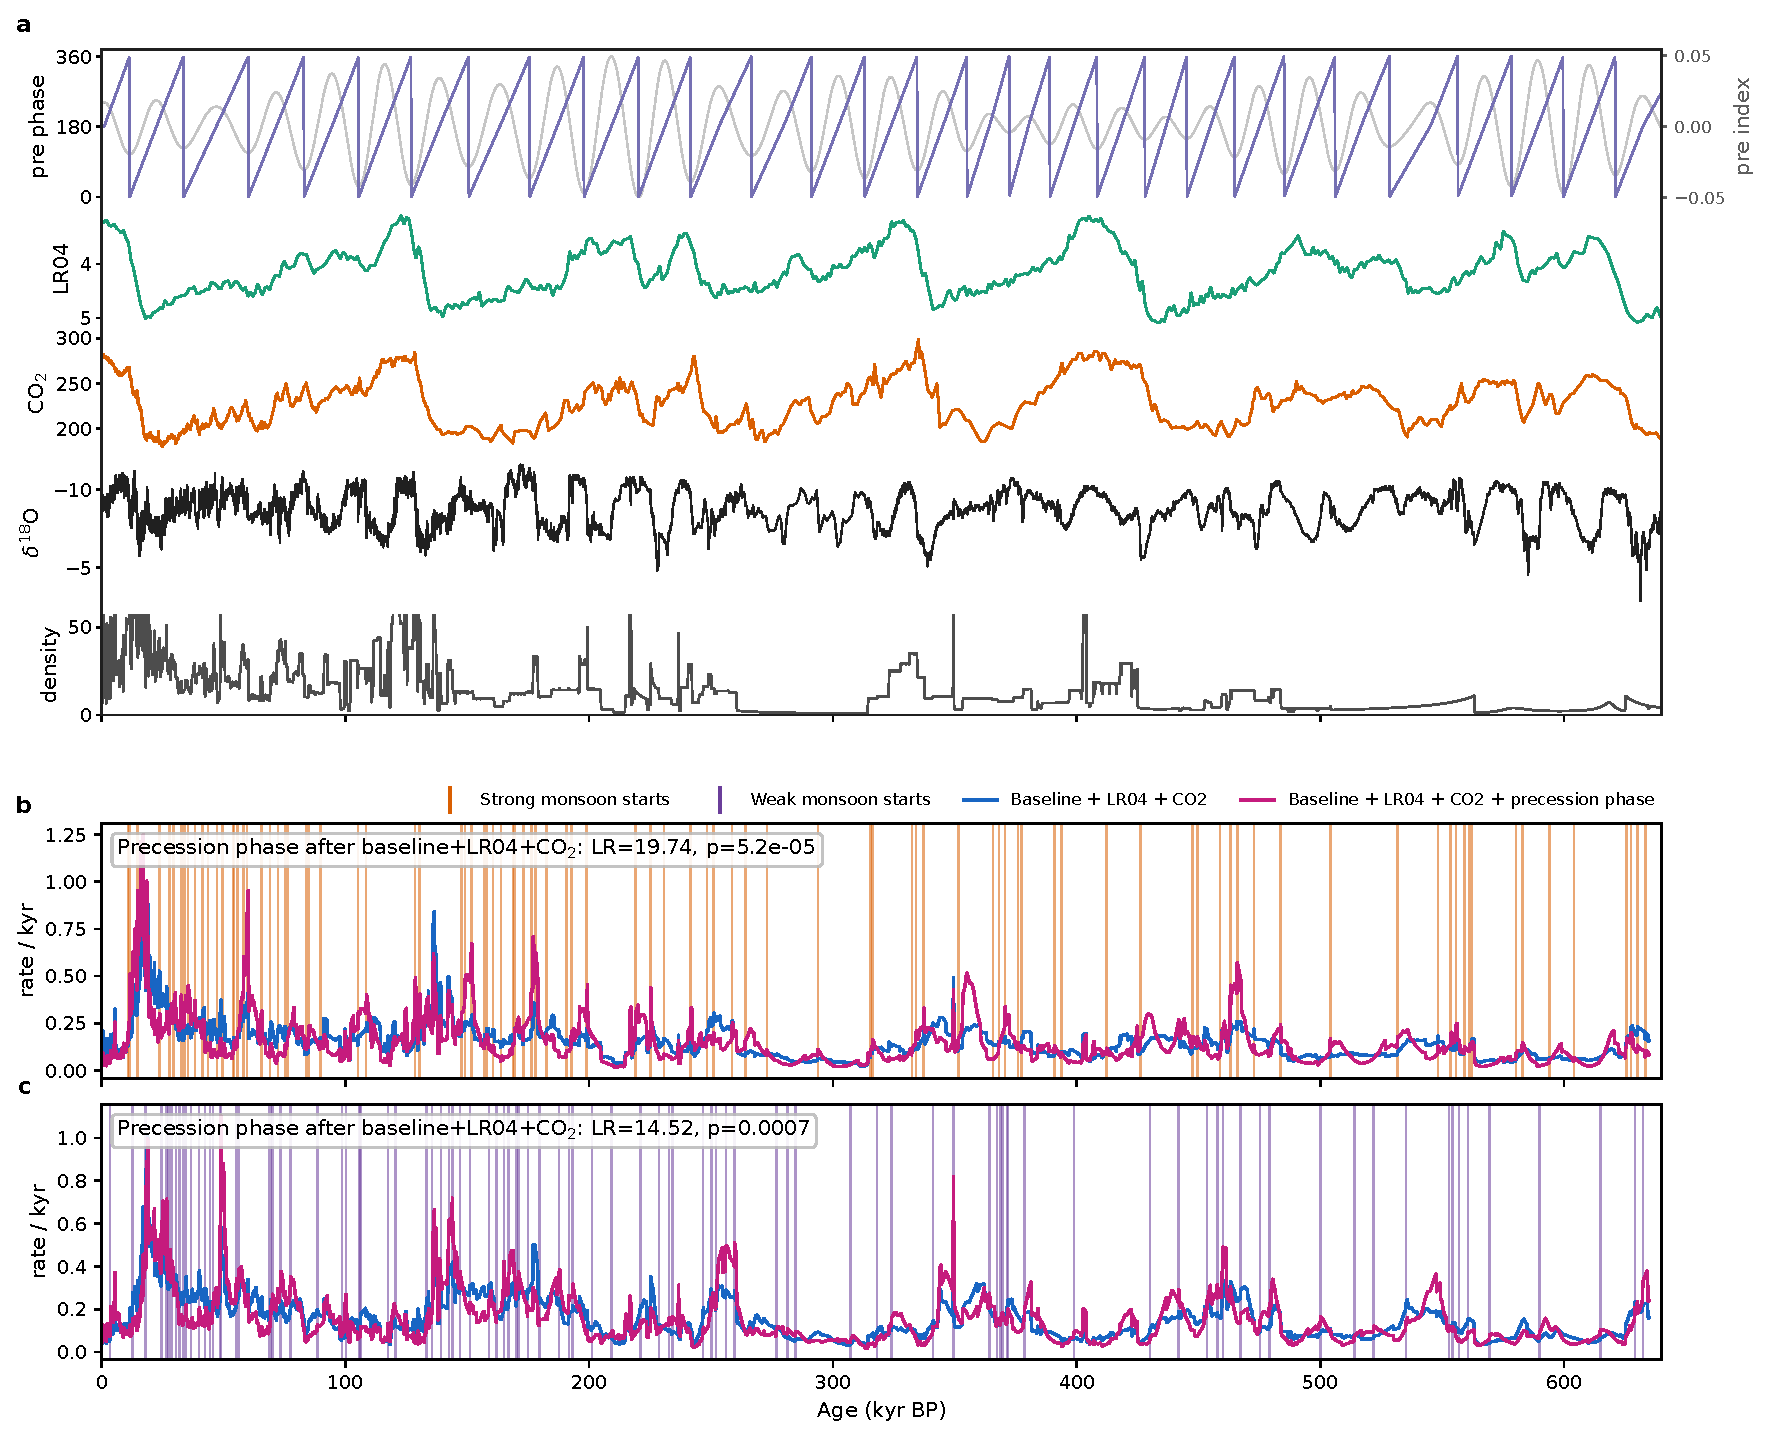
\includegraphics[width=1\textwidth]{../figures/rousseau2023_monsoon_predictive_hazard_history_resolution/fig01_adjusted_inputs_and_fitted_hazards.pdf}
    \caption{
    \textbf{Data and phase framework.}
    (a) Input series used in the adjusted predictive model, including precession phase and raw precession index~\citep{laskar2004long}, LR04 benthic $\delta^{18}\mathrm{O}$~\citep{lisiecki2005pliocene}, atmospheric CO$_2$~\citep{bereiter2015revision}, the Chinese speleothem $\delta^{18}\mathrm{O}$ composite~\citep{cheng2016asian}, and composite sampling density.
    (b) Fitted event rates for strong monsoon starts using the adjusted climate model (event history, data resolution, LR04, and \ce{CO2}), compared with a model additionally including precession phase. Vertical lines mark observed strong-start event bins.
    (c) Same as (b), but for weak monsoon starts. 
    }
    \label{fig:data_phase_framework}
\end{figure}




\section*{Methods}

We analyzed the complete 0.4--4 kyr KS detection-window weak- and strong-monsoon start chronologies identified by Rousseau et al. (2023) from the Chinese speleothem composite of Cheng et al. (2016). This catalogue contains 196 events: 96 strong monsoon starts and 100 weak monsoon starts. All tests were applied independently to the two event catalogues. The adjusted predictive models were fitted on the common support for the event and covariate series, leaving 95 strong starts and 98 weak starts.

Before fitting the predictive models, we performed two supporting event-timing tests. First, a Lohmann-style stationary occurrence test asked whether each start sequence is compatible with a constant-rate random process. Second, circular Rayleigh tests asked whether event phases are uniformly distributed with respect to precession and obliquity. These tests provide diagnostic context but do not adjust for event history, sampling resolution, or glacial background state; details are given in Text S1 and Text S2, and the main diagnostics are summarized in Figure~\ref{fig:randomness_rayleigh}.

The main analysis used a history-conditioned binned Poisson predictive-information framework. The 0--640 kyr BP interval was divided into bins of width \(\Delta t=0.2\) kyr. For bin \(i\), the response was the observed event count \(Y_i\), modeled conditionally on the older event history and external covariates as
\[
Y_i \sim \mathrm{Poisson}(\mu_i),
\qquad
\mu_i = \Delta t_i \lambda_i ,
\]
where \(\lambda_i\) is the event rate per kyr. The log link was applied to the rate,
\[
\log \lambda_i = \beta_0+\mathbf{x}_i^{\top}\boldsymbol{\beta},
\]
or equivalently
\[
\log \mu_i = \log \Delta t_i+\beta_0+\mathbf{x}_i^{\top}\boldsymbol{\beta},
\]
so \(\log \Delta t_i\) entered as an offset. The fitted log-likelihood was
\[
\ell(\boldsymbol{\beta})=
\sum_i
\left[
Y_i\log\mu_i-\mu_i-\log(Y_i!)
\right].
\]

To reduce the risk of attributing catalogue structure to external forcing, every main predictive model was built on an event-process baseline containing two nuisance controls. The first was same-type event history,
\[
H_i=\sum_{t_i<t_j\leq t_i+5\,\mathrm{kyr}} Y_j ,
\]
the number of events of the same type in the immediately older 5 kyr interval. Age increases into the past, so \(H_i\) is a predictable history covariate: the likelihood is interpreted as a product of conditional bin probabilities rather than as an iid Poisson model with independent event histories. The second nuisance control was local sampling resolution of the Cheng et al. composite, estimated as the log local age spacing of the composite \(\delta^{18}\mathrm{O}\) record interpolated to bin centers. This resolution term accounts, in a first-order way, for the possibility that apparent event density covaries with data spacing.

The core model sequence was therefore nested as follows. The event-process baseline included \(H_i\) and sampling resolution. The adjusted climate model added LR04 benthic \(\delta^{18}\mathrm{O}\) and atmospheric \(\ce{CO2}\). The full predictive model further added precession phase:
\[
\log \lambda_i
= \beta_0
+\beta_H H_i
+\beta_R R_i
+\beta_1 \mathrm{LR04}_i
+\beta_2 \mathrm{CO}_{2,i}
+\beta_s \sin\theta_i
+\beta_c \cos\theta_i .
\]
Here \(R_i\) is the scaled log-resolution term and \(\theta_i\) is precession phase at the bin center. Precession phase was defined from the precession-index waveform \citep{laskar2004long} by assigning phase \(0\) to local minima and phase \(\pi\) to local maxima, with linear interpolation of unwrapped phase between adjacent extrema. LR04, \(\ce{CO2}\), and scalar sensitivity predictors were interpolated to bin centers and range-scaled to zero mean and unit observed range. Phase was represented by \(\sin\theta_i\) and \(\cos\theta_i\) because phase is circular.

Models were fitted by maximum likelihood using L-BFGS-B optimization; the stationary model has the analytic maximum-likelihood rate \(N/T\). Models were ranked using sample-size-corrected Akaike information criterion (AICc). Nested models were compared with likelihood-ratio tests,
\[
\mathrm{LR}=2(\ell_\mathrm{full}-\ell_\mathrm{reduced}),
\]
using a chi-square reference distribution with degrees of freedom equal to the number of added coefficients. We also report the same log-likelihood gain as model-based predictive information,
\[
I_{\mathrm{bits/event}}
=
\frac{\ell_\mathrm{full}-\ell_\mathrm{reduced}}
{\ln 2\,N_{\mathrm{events}}}.
\]
The key comparison was precession phase after adjusted climate: the reduced model contained event history, sampling resolution, LR04, and \(\ce{CO2}\), and the full model added the two precession-phase terms. For the two central nested comparisons, we also used reduced-model parametric bootstrap tests that regenerated event catalogues and recomputed same-type history (Text S6).

For models containing \(\sin\theta\) and \(\cos\theta\), the preferred phase and phase-response amplitude were derived from the two coefficients. If the phase component is
\[
\beta_s\sin\theta+\beta_c\cos\theta,
\]
then the phase of maximum fitted rate is
\[
\theta^\ast=\operatorname{atan2}(\beta_s,\beta_c)\ \mathrm{mod}\ 2\pi,
\]
and the amplitude is
\[
A=(\beta_s^2+\beta_c^2)^{1/2}.
\]
The fitted maximum-to-minimum rate ratio over one precession cycle is \(\exp(2A)\).

We also used the same nested-Poisson logic as a lagged predictive-information diagnostic. This analysis was intended to compare temporal alignment among predictors, not to infer a causal response delay. For each driver \(X\) and lag \(\tau\), we compared the event-process baseline with a full model adding \(X(t_i+\tau)\). Positive lag means that the driver was sampled from an older climate state relative to the event bin. Lags from 0 to 20 kyr were scanned in 0.2 kyr steps on a common age support, so that lag comparisons were not affected by changing old-edge coverage. We ran three scans: each driver separately after the event-process baseline; precession phase after LR04 and \(\ce{CO2}\) sampled at the same lag; and precession phase after LR04 and \(\ce{CO2}\) fixed at their own best single-driver lags. Benjamini--Hochberg false-discovery-rate \(q\) values were computed across scanned lags within each dataset and driver family.

Sensitivity experiments tested whether the main result depended on modelling choices or catalogue uncertainty. Additional-forcing tests added Antarctic temperature, obliquity, eccentricity, and \(65^\circ\)N summer-solstice insolation to the full predictive model, here called the extended baseline for sensitivity purposes. We tested each extra forcing individually, all extras jointly, and drop-one contributions within the extended model. Bin-width sensitivity repeated the full model comparison for bin widths of 0.2, 0.4, 0.6, 0.8, and 1.0 kyr. KS-window sensitivity repeated the core tests for the alternative 0.6--4 kyr Rousseau transition catalogue. Composite-age sensitivity generated 500 rank-preserving age-randomized catalogues using an age-uncertainty envelope increasing from 1 kyr at 0 kyr BP to 7.4 kyr at 640 kyr BP---this envelope intentionally adopts conservative values that likely exceed the true composite age uncertainty, because the underlying U--Th dates of individual speleothem records have two-sigma errors on the order of a few hundred years in the youngest portion---and repeated the supporting tests and adjusted predictive-information comparisons for each realization.

\begin{figure}[!htbp]
    \centering
    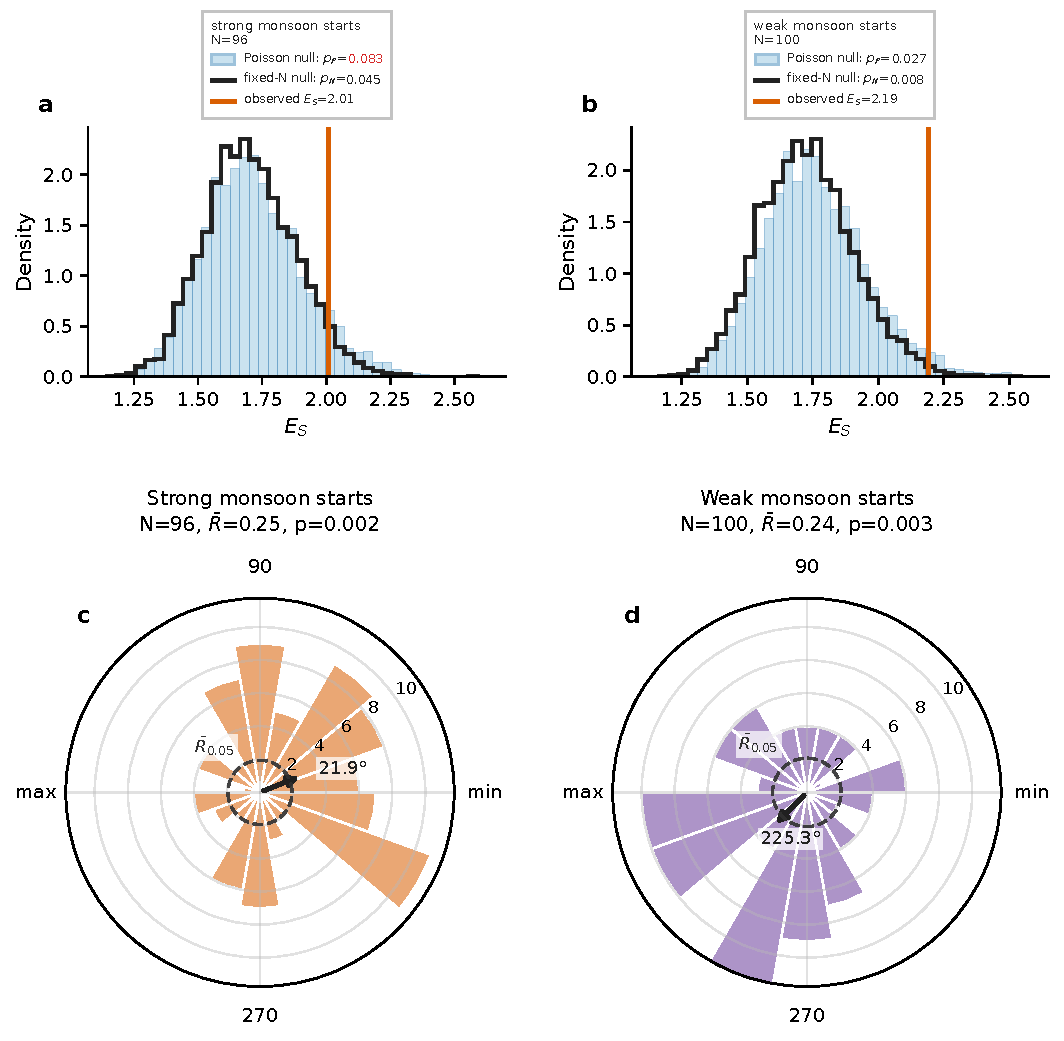
\includegraphics[width=1\textwidth]{../figures/fig02/fig02.pdf}
    \caption{
    \textbf{Event-timing randomness and precession-phase clustering.}
    (a,b) Lohmann-style stationary-event tests for strong and weak monsoon starts, comparing the observed $E_S$ statistic with stationary Poisson and fixed-$N$ null distributions (5000 Monte Carlo realizations each).
    (c,d) Rayleigh tests for clustering of strong and weak monsoon starts in precession phase; arrows show the mean resultant direction and dashed circles mark the $p=0.05$ threshold. Precession index from \citet{laskar2004long}; event catalogue from \citet{rousseau2023reliable}.
    }
    \label{fig:randomness_rayleigh}
\end{figure}




\section*{Results}

The supporting event-timing tests motivate a non-stationary, phase-aware predictive model. The Lohmann-style test shows that the weak monsoon-start sequence is inconsistent with stationary random occurrence under both the unconditional Poisson and fixed-\(N\) nulls, whereas the strong monsoon-start sequence is significant under the fixed-\(N\) null and marginal under the unconditional Poisson null (Figure~\ref{fig:randomness_rayleigh}). Rayleigh tests show significant precession-phase clustering for both strong and weak starts, with mean phases of \(21.9^\circ\) and \(225.3^\circ\), respectively. In contrast, obliquity phases are not significantly clustered for either event type.

The adjusted predictive models show that event history and sampling resolution matter, but they do not remove the precession-phase signal. Relative to a stationary rate, the event-process baseline improved the likelihood for strong starts (\(\mathrm{LR}=16.61\), \(p=2.48\times10^{-4}\)) and weak starts (\(\mathrm{LR}=12.27\), \(p=0.00216\)). Adding LR04+\(\ce{CO2}\) to this baseline further improved prediction for strong starts (\(\mathrm{LR}=13.73\), \(p=0.00104\), \(\Delta\mathrm{AICc}=-9.72\)) and weak starts (\(\mathrm{LR}=21.69\), \(p=1.95\times10^{-5}\), \(\Delta\mathrm{AICc}=-17.68\)). Most importantly, adding precession phase after event history, sampling resolution, LR04, and \(\ce{CO2}\) still improved the model. For strong starts, the likelihood-ratio statistic was \(\mathrm{LR}=19.74\) (\(p=5.16\times10^{-5}\), \(\Delta\mathrm{AICc}=-15.73\), \(0.150\) bits/event). For weak starts, the corresponding statistic was \(\mathrm{LR}=14.52\) (\(p=7.03\times10^{-4}\), \(\Delta\mathrm{AICc}=-10.50\), \(0.107\) bits/event). Reduced-model bootstrap tests gave larger but still significant empirical \(p\) values for both LR04+\(\ce{CO2}\) after the event-process baseline and precession phase after adjusted climate (\(p_\mathrm{boot}<0.003\); Table S3).

The fitted phase preferences agree with the direct Rayleigh tests and show opposite sectors for the two transition directions. In the adjusted model with precession phase but without LR04+\(\ce{CO2}\), strong starts prefer \(20.7^\circ\), close to the Rayleigh mean of \(21.9^\circ\). In the full model, the preferred phase shifts to \(2.1^\circ\), and the maximum-to-minimum rate ratio over the precession cycle is 4.02. Weak starts prefer \(225.1^\circ\) in the baseline-plus-phase model and \(232.8^\circ\) in the full model, with a full-model rate ratio of 3.21. Thus, precession phase contributes information after conditioning on both event-process structure and slow glacial background, and the inferred direction of the phase effect is consistent across independent tests.

The full LR04+\(\ce{CO2}\)+precession-phase model is the main scientific reference model, but the AICc rankings also indicate that LR04 and \(\ce{CO2}\) partly overlap. For strong starts, the lowest AICc model contains LR04 and precession phase but not \(\ce{CO2}\), and the full model ranks second. For weak starts, the lowest AICc model contains \(\ce{CO2}\) and precession phase but not LR04, again with the full model ranking second. Drop-one tests show the same asymmetry: after \(\ce{CO2}\)+precession phase, LR04 is not significant for weak starts, whereas after LR04+precession phase, \(\ce{CO2}\) remains significant for weak starts (\(p=0.0118\)). These results should not be read as a clean separation of ice volume and greenhouse forcing. Rather, LR04 and \(\ce{CO2}\) jointly capture slow glacial background structure, while precession phase remains the clearest orbital timing term after that structure is included.

The additional-forcing sensitivity tests do not identify another independent predictor comparable to precession phase. After the extended baseline model (event history, sampling resolution, LR04, \(\ce{CO2}\), and precession phase) was fitted, adding Antarctic temperature, obliquity, eccentricity, or \(65^\circ\)N summer-solstice insolation one at a time did not significantly improve the strong-start model (\(p=0.452\)--0.953) or the weak-start model (\(p=0.127\)--0.877). Adding all four extra forcings jointly also failed to improve prediction for strong starts (\(p=0.932\), \(\Delta\mathrm{AICc}=+7.20\)) or weak starts (\(p=0.455\), \(\Delta\mathrm{AICc}=+4.40\)). The only suggestive but non-significant case is \(65^\circ\)N insolation for weak starts, which slightly lowers AICc when added alone (\(\Delta\mathrm{AICc}=-0.32\)) and in the drop-one test (\(\Delta\mathrm{AICc}=-1.20\)), but has likelihood-ratio \(p=0.127\) and \(p=0.073\), respectively. We therefore treat this as weak sensitivity, not as evidence for an additional independent forcing.

The bin-width, KS-window, and age-uncertainty sensitivity experiments support the robustness of the precession-phase result. Across bin widths from 0.2 to 1.0 kyr, precession phase after adjusted LR04+\(\ce{CO2}\) remains significant for both event catalogues. Strong-start preferred phases stay between \(2.1^\circ\) and \(5.5^\circ\), and weak-start preferred phases stay between \(232.8^\circ\) and \(234.5^\circ\); all phase shifts relative to the 0.2 kyr baseline are less than \(3.4^\circ\). Using the narrower 0.6--4 kyr KS-window catalogue also preserves Rayleigh precession clustering and the adjusted precession-phase likelihood-ratio result for both strong and weak starts. Finally, in 500 age-randomized catalogues, the precession-phase term after adjusted LR04+\(\ce{CO2}\) remains significant in 100\% of realizations for both event types. Rayleigh precession clustering remains significant in 99.6\% of strong-start and 99.0\% of weak-start age-randomized catalogues. The main sensitive result is not the precession signal, but the strong-start Lohmann randomness test, whose fixed-\(N\) significance survives in only 49.8\% of age-randomized catalogues.

The single-driver lagged predictive-information scan is summarized in Figure~\ref{fig:lagged-single-driver-info}.

\begin{figure}[!htbp]
    \centering
    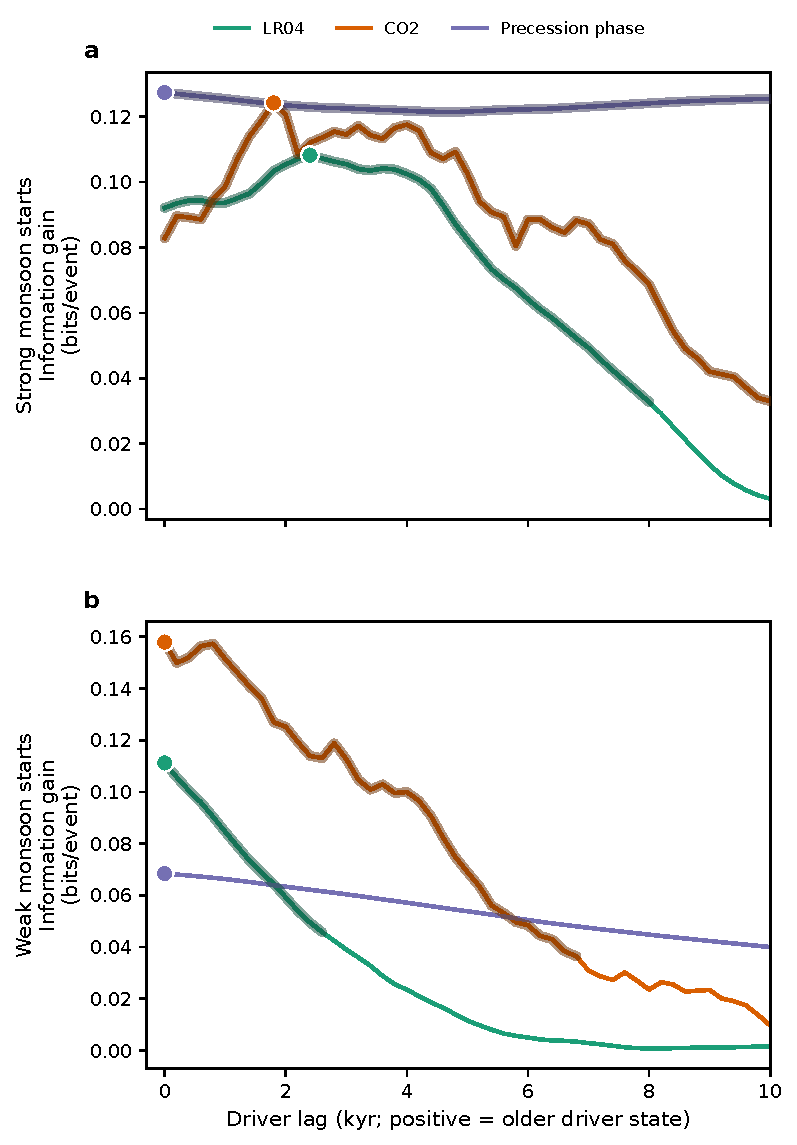
\includegraphics[width=0.52\textwidth]{../figures/rousseau2023_monsoon_lagged_te_predictive_info/fig01_single_driver_lagged_information.pdf}
    \caption{\textbf{Lagged predictive information from individual drivers.}
    Model-based predictive-information gain, expressed as bits per event, from adding lagged LR04~\citep{lisiecki2005pliocene}, \ce{CO2}~\citep{bereiter2015revision}, or precession phase~\citep{laskar2004long} to the event-process baseline containing same-type event history and sampling resolution.
    (a) Strong monsoon starts.
    (b) Weak monsoon starts.
    Positive lags indicate that the driver is sampled from an older climate state relative to the event bin.}
    \label{fig:lagged-single-driver-info}
\end{figure}



\section*{Discussion}
The main result is that precession phase organizes the probability of DO-like Asian monsoon transitions after several conservative adjustments. The adjusted baseline controls for recent same-type event occurrence and for local composite sampling resolution, so the precession signal is not simply a consequence of event clustering or higher apparent detection density in better-resolved parts of the record. LR04 and \(\ce{CO2}\) then account for slow glacial background state. The persistence of the precession-phase term after all of these controls means that the result is best stated as conditional predictive information: given event history, sampling resolution, LR04, and \(\ce{CO2}\), precession phase still improves prediction of event occurrence.

The lagged predictive-information scan helps interpret what is and is not being measured. For strong starts, the best single-driver lags are 2.4 kyr for LR04, 1.8 kyr for \(\ce{CO2}\), and 0 kyr for precession phase (Figure~\ref{fig:lagged-single-driver-info}). For weak starts, the best single-driver lags are 0 kyr for LR04, 0.8 kyr for \(\ce{CO2}\), and 0 kyr for precession phase, although the single-driver weak-start precession scan is weaker after false-discovery-rate correction. In the stricter conditional tests, precession phase remains informative after LR04 and \(\ce{CO2}\) are included either at the same lag or at their best single-driver lags. The strongest conditional phase signal occurs at 0 kyr for strong starts and at 0--0.8 kyr for weak starts. These near-zero lag maxima should be read as contemporaneous orbital-phase organization, not as resolved causal delays: precession phase is a smooth deterministic orbital variable, and the event catalogue is sparse. The diagnostic nevertheless supports a useful separation: LR04 and \(\ce{CO2}\) behave as slowly varying background-state predictors, whereas precession phase behaves more like an orbital-seasonal transition-window variable.

A conservative physical interpretation is that the predictive model separates two aspects of boundary forcing. LR04 and \(\ce{CO2}\) summarize slowly evolving glacial background conditions, including ice volume, deep-ocean temperature, greenhouse forcing, and the boundary-state controls that can alter North Atlantic sea ice, freshwater routing, and AMOC stability \citep{lisiecki2005pliocene,zhang2017abrupt,vettoretti2022atmospheric,zhang2021direct}. Precession phase, by contrast, indexes the position of perihelion relative to the seasonal cycle and therefore the seasonal geometry of low-latitude insolation forcing \citep{berger1978long,berger1991insolation}. This distinction matters for Asian speleothem records, which integrate abrupt North Atlantic-linked hydroclimate changes and orbitally paced monsoon dynamics \citep{cheng2016asian,corrick2020synchronous,xie2023contributions}. The result therefore favors a background-susceptibility plus orbital-phase-organization view, not deterministic astronomical triggering of individual transitions.

The different preferred phases for strong and weak starts suggest that precession does more than modulate the overall amplitude of millennial variability. In the COSMOS experiments of \citet{zhang2021direct}, changes in eccentricity-modulated precession under intermediate glacial boundary conditions can move the AMOC from a monostable state into a self-sustained DO-like oscillatory regime. Their precession-only experiment links this behavior to seasonally specific low-latitude forcing that modifies tropical North Atlantic hydroclimate and salinity, with subsequent interaction with subpolar sea-ice--ocean feedbacks. Our proxy result is consistent with that dynamical picture in one important respect: precession phase remains associated with transition probability after glacial background predictors are included. It also adds a constraint not provided by amplitude-envelope studies. Strong starts cluster near the precession-index minimum sector, whereas weak starts cluster in the opposite half-cycle. This should not be read as exact \(180^\circ\) antiphasing: the precise preferred angles vary between the Rayleigh, baseline-plus-phase, and fully adjusted estimates, and transition probability need not peak exactly at precession-index extrema. We therefore interpret the contrast as an asymmetric, direction-dependent phase organization of entering versus leaving strong-monsoon states linked to Greenland interstadial-like conditions, rather than as exact antiphased astronomical pacing.


The weak additional contribution of obliquity and \(65^\circ\)N summer-solstice insolation should be interpreted narrowly. Obliquity may still influence MCV amplitude or the background stability of DO-like regimes \citep{sun2021persistent,hodell20231,zhang2021direct,malmierca2023dansgaard}. Likewise, \(65^\circ\)N summer-solstice insolation remains dynamically relevant to high-latitude ice and sea-ice processes. Our result is more specific: within this event catalogue and this adjusted predictive model, neither obliquity nor a scalar high-latitude summer-solstice index adds a separable event-timing signal once event history, sampling resolution, LR04, \(\ce{CO2}\), and precession phase are included. The weak AICc improvement from \(65^\circ\)N insolation for weak starts is therefore a sensitivity flag, not a basis for replacing the phase result.

Several limitations should be kept in view. First, the event catalogue depends on the Rousseau et al. transition-detection procedure applied to a composite speleothem record. The precession-phase result is stable across the two KS-window catalogues, across bin widths, and across the approximate age-randomized catalogues used here, but a full ensemble of speleothem age models would provide a stronger uncertainty propagation. In defence of the detection procedure, the KS parameters were optimized via ROC analysis against independently known events, and the method correctly identifies 23 of 24 Greenland DO events in the last glacial \citep{rousseau2023reliable}. The opposite-phase structure across the two transition types is difficult to explain as a window-dependent artifact because the same procedure applied to different KS windows yields indistinguishable phase preferences. Additionally, the splicing of different speleothem records in the Cheng et al. composite is a potential source of artefactual transitions, though the stable phase results across detection windows and age perturbations argue against a dominant splice-related bias. Second, speleothem \(\delta^{18}\mathrm{O}\) is not a direct local precipitation amount. It integrates upstream rainout, moisture-source changes, circulation pathways, seasonality, and regional hydroclimate effects \citep{liu2014chinese, cheng2021orbital, zheng2022decoupled}. The terms ``strong'' and ``weak'' monsoon states are therefore best understood as large-scale speleothem-recorded monsoon-system states rather than simple local rainfall anomalies. This caveat is particularly relevant in light of moisture-source results such as \citet{xie2023contributions}, which show that orbital precipitation changes can involve changing terrestrial and oceanic source contributions.

At 0.150 bits/event, knowledge of precession phase reduces event-timing uncertainty by about 15\% relative to the baseline model, indicating that while the signal is statistically robust, most of the event-timing variance remains unexplained---consistent with a stochastic threshold-crossing mechanism rather than deterministic forcing. Third, the Poisson predictive model is an intentionally simple statistical approximation. The 0.2 kyr bin width keeps the within-bin constant-rate assumption conservative, and the bin-width sensitivity test shows that the qualitative results are stable up to 1 kyr. Sparse-bin diagnostics show no excess-zero or overdispersion signal relative to the fitted Poisson models, and bootstrap likelihood-ratio tests support the main comparisons (Text S6). Still, the model assumes conditional independence after the included history and covariate terms, does not explicitly represent event-duration dynamics, and uses a limited set of background predictors. The likelihood-ratio tests therefore establish statistical association and predictive improvement, not a complete dynamical mechanism. Fourth, covariates such as precession phase, summer insolation, eccentricity, and ice-volume-related background state are not independent components of the climate system. The sensitivity results show that additional variables do not improve the selected extended baseline in this model, but they should not be interpreted as excluding indirect pathways through which obliquity, eccentricity, or ice sheets influence MCV.

Despite these caveats, the event-based signal is robust across several complementary tests. The stationary tests show that the transition sequences are not fully compatible with simple random occurrence. The Rayleigh tests show direct precession-phase clustering. The adjusted predictive models show that precession phase remains informative after event history, sampling resolution, LR04, and \(\ce{CO2}\) are included. The sensitivity experiments show that this conclusion is stable to bin width, KS detection window, and approximate age perturbation, and is not replaced by AT, obliquity, eccentricity, or \(65^\circ\)N summer-solstice insolation as independent additions. Together, these results point to precession-phase organization of abrupt monsoon-transition probability, superimposed on slower glacial background modulation.

\section*{Conclusions}

This study tests whether the timing of DO-like Asian monsoon transitions in the 0--640 kyr BP Chinese speleothem composite is organized by orbital phase. Strong and weak monsoon starts show significant and opposite precession-phase preferences. These preferences persist in a history-conditioned binned Poisson predictive-information model after conditioning on same-type event history, Cheng composite sampling resolution, LR04, and atmospheric \(\ce{CO2}\). Strong starts preferentially occur near the precession-index minimum sector, while weak starts occur in the opposite half-cycle. Additional forcings, including obliquity, eccentricity, Antarctic temperature, and \(65^\circ\)N summer-solstice insolation, do not add comparable independent predictive power in this framework. The result is stable across bin-width, KS-window, and approximate age-uncertainty sensitivity tests. A complementary lagged predictive-information scan suggests that precession-phase information is strongest at near-zero lag, consistent with phase organization at the time of transition rather than a resolved causal delay. We therefore interpret the results as evidence that precession phase helps organize the timing and direction of speleothem-recorded abrupt monsoon transitions, while glacial background state modulates the system's susceptibility to such transitions. This event-timing perspective extends earlier work on orbital modulation of continuous speleothem \(\delta^{18}\mathrm{O}\) and MCV amplitude, and provides a statistical target for transient climate-model experiments that seek to explain how orbital forcing and glacial boundary conditions interact to pace abrupt hydroclimate changes.


\section*{Data Availability}

All data used in this study are from previously published sources: the Chinese speleothem composite \citep{cheng2016asian}, the 196 abrupt transition catalogue \citep{rousseau2023reliable}, LR04 benthic $\delta^{18}$O stack \citep{lisiecki2005pliocene}, atmospheric CO$_2$ from EPICA Dome C \citep{bereiter2015revision}, and orbital solutions \citep{laskar2004long}. The analysis code is available at \url{https://github.com/Peisong-Zheng/DO_warming}.

\section*{Acknowledgements}

This work was supported by the UKRI Centre for Doctoral Training in Application of Artificial Intelligence to the study of Environmental Risks (reference EP/S022961/1).

\section*{Competing Interests}

The authors declare no competing interests.

\bibliographystyle{agu}
\bibliography{reference}
\end{document}
